\documentclass[10pt,twocolumn]{IEEEtran11}

\usepackage{comment}
\usepackage{times}
\usepackage{epsfig}
\usepackage[T1]{fontenc}
\usepackage[utf8]{inputenc}
\usepackage{graphicx}
\usepackage{subfigure}
\usepackage{url}
\def\BibTeX{{\rm B\kern-.05em{\sc i\kern-.025em b}\kern-.08em
    T\kern-.1667em\lower.7ex\hbox{E}\kern-.125emX}}

\oddsidemargin -15pt
\evensidemargin -15pt
\leftmargin 0 pt
\topmargin -35pt
\textwidth = 6.9 in
\textheight = 9.1 in

\newcommand{\itembase}{\setlength{\itemsep}{0pt}}
\newcommand{\eg}{{\it e.g., }}
\newcommand{\ie}{{\it i.e., }}
\graphicspath{{FIG/}}

\begin{document}
\bibliographystyle{IEEE}

\title{\Large \bf CIS 632 - Technical Report: Twitter Project
%\thanks{
}

\author{Adam Bates and Lara Letaw\\
Department of Computer \& Information Science\\
University of Oregon\\
\textit{\{amb,zephron\}@cs.uoregon.edu}}

\maketitle
% You have to do this to suppress page numbers.  Don't ask.
%\pagestyle{empty}
%\begin{abstract}
%Write your abstract here
%\end{abstract}

%\begin{keywords} 
%Keywords
%\end{keywords}

%\section{Introduction}
%Twitter is a microblogging and social networking servive that allows its users to send short, one-to-many messages called \textit{tweets}.  Like many online social networks, users can opt-in to viewing other users' messages \textit{following} them, creating a customized content stream.  The act of following is an implicit endorsement of another user on the network.  It can be inferred that the user being followed is of interest to another user on the network.  These interactions constitute a networked system through which users connect and message propagate.

In order to gain a better understanding of Twitter, it is necessary to investigate the nature of this network.  This information can be used when considering design decisions or allocating resources within Twitter or other future social networks.  While Twitter is innovative in the manner in which it distributes messages, a great deal of this profiling must take place at the user-level network.

Twitter, like many other online social networks, present a novel opportunity to study interactions between people.  Through them, it becomes possible to easily quantify the activities of millions.  The simple and open structure of the Twitter network is particularly well-suited for this purpose.  As each user account is associated with a variety of attributes, there a variety of methods to approach this task.  The work we present here establishes a framework for further analysis.

There are many commonly held intuitions regarding influence that can be proved, disproved or measured through analysis of Twitter.  For example, it is a commonly held belief that activity in states such as California and New York is of a higher culturally relevance than the activity in other states.  As each user account is associated with a location field, it is possible to use the Twitter network to measure the influence of these allegedly trend-setting states.  Other, subtler biases can also be identified and evalued in the same manner.

A defining aspect of Twitter that lends itself to research is that all activity defaults to public.  Each user's messages are visible unless they explicitly change their privacy setting.  Although tweets can be protected, all other information associated with an account visible to all.  Using this publicly available connectivity information, it is possible to make broad assessments of connectivity within the Twitter community.

Given the massive size and continued growth of Twitter, capturing a complete snapshot of the network is an increasingly unrealistic endeavor.  To make matters worse, Twitter imposes prohibitive rate limitations on access to many of its network measurement resources.  It is therefore necessary to obtain a representative and meaningful sampling of the network before analysis begins.

One possible option is to take a random sample of a small percentage of Twitter accounts and activity.  Inspection of this random sample's attributes would lead to a representative view, but not necessarily a meaningful one.  The users of greatest interest are small in number and some of their attributes will have extreme values.  A random sample is not likely to capture these users' impact on the network.

It is also possible to conduct a biased sampling.  Here, interesting users with extreme user attribute values are specifically targetted for measurement.  If good metrics are used to assess influence, this will ensure that important user accounts are not crowded out by unimportant ones.  Of course, this leads to data that is less representative than a random sampling.  It can be observed that there is a natural trade-off between these two goals.

Our approach finds a healthy compromise between these competing priorities by starting with a biased sample and then performing a mult-hop crawl across a small piece of the network to conduct further sampling.  This crawl creates a snapshot of a part of Twitter that is acceptably representative while simultaneously ensuring that rare users are acceptably prominent.  We establish that our snapshot is representative by comparing its profile to the profile of a true random sample.

STILL NEED TO PUT A SUMMARY OF OUR WORK APPROACH AND MAIN FINDINGS HERE (AS PER REZA'S REPORT DESCRIPTION)

The rest of this paper is organized as follows.  We outline our data collection process in section \ref{sec:datacollection}.  In section \ref{sec:methodology}, we present our method for evaluating connectivity bias within the Twitter network.  Analysis of our results is contained in section \ref{sec:analysis}.  We review some of the related work in section \ref{sec:relatedwork}.  Section \ref{sec:conclusion} concludes the paper.

\section{Motivation}  
Twitter is a not just a new technology;  it is also a new form of communication.  Although there is a variety of ongoing Twitter-related research, there are a myriad of remaining potential approaches.  There are still open questions regarding influence within the Twitter network.  We hope to evaluate influence as it relates to the various attributes associated with a user account.  

\section{Related Work}  
One of Twitter's core functions is the analysis of individual messages to determine trending topics.  As such, Twitter is capable of acting a cultural barometer.  A variety of studies have attempted to answer the question of how information spreads within the Twitter network.  Investigations have included spam, the meme life cycle, and news discovery and explanation.\\\\
A variety of Twitter-related work has been conducted over the past several years.  The majority of this work focuses on the analysis and propagation of individual messages as they spread through the network.  Cheng \textit{et al} have used tweets to attempt to geo-locate users based on the content of their messages ~\cite{CCL10}.  Lerman and Ghosh have studied Digg and Twitter to measure news items' lifespan and speed within social networks ~\cite{LG10}.  Sadikov and Martinez have conducted similar work, chosing instead to focus on URL and tag propagation ~\cite{SM09}.\\
It is only reasonable that message-level analysis has captured the attention of the research community.  After all, the novelty of modern social networks is largely that they are a new medium for the spread of information.  For the purposes of assessing influence, however, message-level analysis does not tell the whole story.  Much of this work lies in predictive message filtering or spotting trending phrases.  This is not perfectly suited for the task of broadly determining who is influencing who.  Instead, we ask a much simpler question -- what type of people are users choosing to listen to?\\
For this, we turn to user-level analysis.  When a user choses to opt-in to another user's tweet stream, this says much more about influence than the propagation of individual messages.  This idea of influence through followers is a truth that rests at the very core of Twitter, one that can be plainly seen by visiting any user's page and making note of the prominently displayed ``Follower'' and ``Following'' numbers.  Our contribution will be to take this fundemental concept and cross-reference it with various user attributes in an attempt to make more general claims about the nature of influence in the Twitter network.

\section{Methodology}
\subsection{Approaching Attribute Analysis}

Paragraph: Describe the manner in which we approach each attribute.  Explain that for some attributes with a small number of options it is easy to investigate all simultaneously.  Explain for the range options that we created logarithmic bins to accurately capture our extreme uses.\\

Paragraph: Explain how Location was an entirely different animal because it is a freely entered text field.  A large number of users do not put valid locations in this field.  For the users that do, those options are often difficult to parse.\\

Paragraph:  Mention that some attributes were not considered at all.  Explain the attributes that were not considered because they were completely irrelevant (bg color)  Explain the attributes that were not considered because their values were not sufficiently heterogenous (verified).\\

Paragraph: Mention the simple random survey of records that was performed, the percentage of users with no entry, the percentage of users with an indecipherable entry, etc.\\

Paragraph: Explain that it was decided to evaluate location based on state.\\

\subsection{Evaluation}

Paragraph: Explain the basic challenge of deriving bias from the measured following patterns.

Paragraph: Explain the method for calculating the expected connectivity in a randomized, bias-free version of our subgraph.  Include formula.

Paragraph: Explain the method for calculating bias from this value and the measured values.  Include formula.



\section{Evaluation}
We will our connectivity dataset and crawl across it to find a particularly great subgraph.  If time allows, we will attempt to restore and expand the incomplete information within this subgraph.  We will then create overlays of this subgraph using different user attributes.  We will analyze the directional nature of these subgraph overlays.

\begin{figure}
 \centering
 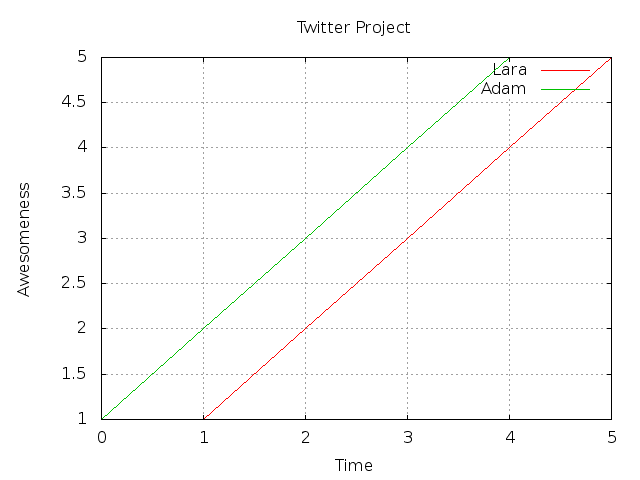
\includegraphics[bb=0 0 640 480,scale=.25]{./images/evidence.png}
 % evidence.png: 640x480 pixel, 72dpi, 22.58x16.93 cm, bb=0 0 640 480
 \caption{This is what a graph looks like.}
 \label{Figure 1:}
\end{figure}

\subsection{Assessing the validity of our subgraph}

\section{Timetable}
\textit{(To be revised as needed.)}

\subsection*{January 3-23}
\begin{itemize}
\item{Developed project proposal}
\item{Determined feasibility of data collection}
\item{Built subgraphs of core users}
\item{Collected user data for all core and leaf users}
\end{itemize}

\subsection*{January 24-30}
\begin{itemize}
\item{Ensure data set is complete as far as user attribute collection}
\item{Perform preliminary user attribute distribution analysis}
\item{Bridge subgraph connections}
\item{Determine feasibility of collecting missing friends and followers}
\item{Acquire random data sets}
\item{Build baskets for which baskets are already enumerated}
\end{itemize}

\subsection*{January 31 - February 5}
\begin{itemize}
\item{Formalize method for characterizing connectivity}
\item{Determine basket filters for variable attributes}
\item{Determine basket sizes for continuous attributes}
\item{Merge subgraph and user attribute databases}
\end{itemize}

\subsection*{February 6-12}
\begin{itemize}
\item{Select most informative basket configurations}
\item{Select most interesting user attributes}
\item{Determine if there are any interesting composite attributes to inspect}
\item{Begin creating connectivity visualizations}
\end{itemize}

\subsection*{February 13 - March 1}
\begin{itemize}
\item{Continue to refine and polish attribute basketing and assessment}
\item{Complete first draft of research paper}
\end{itemize}

\subsection*{March 2-13}
\begin{itemize}
\item{Complete final draft of research paper}
\end{itemize}

\subsection*{March 14}
\begin{itemize}
\item{Submit final research paper}
\item{Give project presentation}
\end{itemize}

\onecolumn
\section{User Attributes}
Below are the user attributes we plan to examine in our analyses. In reference to number of baskets, \textit{varied} means we will experiment with different numbers of baskets.\\

\noindent \begin{tabular}[t]{| p{1in} | p{1.75in} | p{1in} | p{1in} | p{1.25in} |}
\hline
\textbf{Attribute} & \textbf{Description} & \textbf{\# of Baskets (Core)} & \textbf{\# of Baskets (All)} & \textbf{Values}  \\ \hline
Location & User-reported geographic location. & 3481 & 3481 & U.S. state code \\ \hline
Protected & If true, only approved followers may see the user's tweets & 2 & 2 & true, false \\ \hline
Followers Count & Number of users who track this user's tweets & 2116 & 2116 & integer \\ \hline
Friends Count & Number of users this user follows & 2116 & 2116 & integer \\ \hline
Account age & Difference between account creation date and current date & 169 & 169 & time \\ \hline
\begin{comment}
UTC Offset & Time offset from Coordinated Universal Time & 34 & 34 & integer \\ \hline
Time Zone & Logitudinal region & 141 & 143 & time zones  \\ \hline
\end{comment}
Geo-Enabled & GPS meta data is included on tweets & 2 & 2 & true, false \\ \hline
Verified & Twitter has verified the identity of the user, currently used for Twitter partners and advertisers & 2 & 2 & true, false \\ \hline
Statuses Count & Number of tweets & 2116 & 2116 & integer  \\ \hline
Language & User's chosen language & 7 & 7 & en, de, it, es, ja, fr, ko \\ \hline
Contributors Enabled & If enabled, multiple users can tweet from this account & 2 & 2 & true, false \\ \hline
Listed Count & Number of lists that include this account & 2116 & 2116 & integer \\ \hline
Show All Inline Media & Display photos and videos of other users, not just friends & 2 & 2 & true, false \\ \hline
URL & This user posted a URL & 2 & 2 & true, false \\ \hline
Is Translator & User has signed up to translate other people's tweets  & 2 & 2 & true, false \\ \hline
%Status Source & Where the most recent status was tweeted from & 5,144 & 39,566 & (none), web, various URLs \\ \hline  
\end{tabular}

\section{Dataset Profile}

\textit{Available users} are those for which user profile data was successfully collected.  Unavailable users are those for whom an attempt to acquire user attributes resulted in a \textit{404 Not Found} error.  We assume these user accounts are closed.\\ 
\begin{tabular}[t]{| l | l |}
\hline
Users & 17,688,493  \\ \hline
Available Users & 17,475,570 (98.8\%) \\ \hline
Unavailable Users & 212,923 (1.2\%) \\ \hline
Core Users & 242,275 \\ \hline
Available Core Users & 238,323 (98.8\% of core) \\ \hline
Unavailable Core Users & 3,952 (1.2\% of core) \\ \hline
\end{tabular}

\subsection{Subgraphs}
\textit{Graph edges} refers to the connections between core users and any other user.\\\\
\begin{tabular}{| l | l | }
\hline
Users is Subgraph 1 & 15,548,091 \\ \hline
Available Users is Subgraph 1 & 15,363,277 \\ \hline
Core Users in Subgraph 1  & 194,004 \\ \hline
Remaining Core Users  & 48,267 \\ \hline
Remaining Subgraphs  & 46,403 \\ \hline
Connections to Subgraph 1  & 46,924 \\ \hline
Total Connected Users & 240,932 \\ \hline
\end{tabular}

\subsection{Boolean User Attributes}
Attributes whose values are either \textit{true} or \textit{false}.\\\\
\begin{tabular}{| l | l | l |}
\hline
\textbf{Attribute} & \textbf{\# True (Core)} & \textbf{\% True (Core)} \\ \hline
Protected & 8,517 & 3.575  \\ \hline
Geo-Enabled & 58,432 & 24.518 \\ \hline
Verified & 119 & 0.050 \\ \hline
Contributors Enabled & 7 & 0.003 \\ \hline
Show All Inline Media & 18,870 & 7.918 \\ \hline
URL & 118,364 & 49.665 \\ \hline
Is Translator & 72 & 0.030 \\ \hline
\end{tabular}

\subsection{Enumerated User Attributes}
Attributes for which there are a relatively small number of values, other than boolean values.
\subsubsection{Language}
Percentage of users per language.\\\\
\begin{tabular}{| l | l | l | l | }
\hline
\textbf{Language Code} & \textbf{Language} & \textbf{\# (Core)}  & \textbf{\% (Core)} \\ \hline
en & English & 173,782 & 72.919 \\ \hline
ja & Japanese & 44,499 & 18.672 \\ \hline
es & Spanish & 16,210 & 6.802 \\ \hline
de & German & 1,560 & 0.655 \\ \hline
fr & French & 1,222 & 0.513 \\ \hline
it & Italian & 713 & 0.299 \\ \hline
ko & Korean & 337 & 0.141 \\ \hline
\end{tabular}

\subsubsection{UTC Offset}
\begin{tabular}{| l | l | l |}
\hline
\textbf{UTC Offset} & \textbf{\# (Core)} & \textbf{\% (Core)} \\ \hline
(none)	&	38287	&	16.065	\\ \hline
32400	&	36551	&	15.337	\\ \hline
-18000	&	26196	&	10.992	\\ \hline
-10800	&	25001	&	10.490	\\ \hline
-28800	&	23344	&	9.795	\\ \hline
-21600	&	17830	&	7.481	\\ \hline
-14400	&	12698	&	5.328	\\ \hline
25200	&	10425	&	4.374	\\ \hline
-36000	&	10162	&	4.264	\\ \hline
3600	&	9607	&	4.031	\\ \hline
0	&	7067	&	2.965	\\ \hline
-25200	&	4360	&	1.829	\\ \hline
28800	&	4065	&	1.706	\\ \hline
-32400	&	3573	&	1.499	\\ \hline
-16200	&	2685	&	1.127	\\ \hline
7200	&	1908	&	0.801	\\ \hline
36000	&	1286	&	0.540	\\ \hline
10800	&	1054	&	0.442	\\ \hline
19800	&	717	&	0.301	\\ \hline
43200	&	322	&	0.135	\\ \hline
-39600	&	236	&	0.099	\\ \hline
14400	&	213	&	0.089	\\ \hline
18000	&	163	&	0.068	\\ \hline
12600	&	138	&	0.058	\\ \hline
34200	&	103	&	0.043	\\ \hline
-7200	&	100	&	0.042	\\ \hline
21600	&	91	&	0.038	\\ \hline
-12600	&	57	&	0.024	\\ \hline
46800	&	24	&	0.010	\\ \hline
-3600	&	20	&	0.008	\\ \hline
39600	&	19	&	0.008	\\ \hline
16200	&	9	&	0.004	\\ \hline
23400	&	7	&	0.003	\\ \hline
20700	&	5	&	0.002	\\ \hline
\end{tabular}
\vspace{2.5in}

\subsubsection{Time Zone}
Only the top 100 time zones are shown here.\\
\begin{tabular}{| l | l | l | l | l | l |}
\hline
\textbf{Time Zone} & \textbf{\# (Core)} & \textbf{\% (Core)} & \textbf{Time Zone} & \textbf{\# (Core)} & \textbf{\% (Core)} \\ \hline
(none)	&	38287	&	16.065	&	Kyiv	&	215	&	0.090	\\ \hline
Tokyo	&	30332	&	12.727	&	Brussels	&	214	&	0.090	\\ \hline
Pacific Time (US \& Canada)	&	23280	&	9.768	&	Monterrey	&	214	&	0.090	\\ \hline
Brasilia	&	15997	&	6.712	&	Lima	&	194	&	0.081	\\ \hline
Central Time (US \& Canada)	&	15327	&	6.431	&	Copenhagen	&	183	&	0.077	\\ \hline
Eastern Time (US \& Canada)	&	15066	&	6.322	&	Riyadh	&	178	&	0.075	\\ \hline
Santiago	&	12131	&	5.090	&	Abu Dhabi	&	173	&	0.073	\\ \hline
Hawaii	&	10162	&	4.264	&	Athens	&	164	&	0.069	\\ \hline
Quito	&	10152	&	4.260	&	Bucharest	&	151	&	0.063	\\ \hline
Jakarta	&	9334	&	3.917	&	West Central Africa	&	151	&	0.063	\\ \hline
Greenland	&	7968	&	3.343	&	Warsaw	&	148	&	0.062	\\ \hline
London	&	5968	&	2.504	&	Perth	&	145	&	0.061	\\ \hline
Mountain Time (US \& Canada)	&	3826	&	1.605	&	Chennai	&	144	&	0.060	\\ \hline
Amsterdam	&	3600	&	1.511	&	Auckland	&	139	&	0.058	\\ \hline
Alaska	&	3573	&	1.499	&	Tehran	&	138	&	0.058	\\ \hline
Osaka	&	3509	&	1.472	&	Guadalajara	&	133	&	0.056	\\ \hline
Caracas	&	2685	&	1.127	&	Cairo	&	130	&	0.055	\\ \hline
Seoul	&	1912	&	0.802	&	Vienna	&	126	&	0.053	\\ \hline
Mexico City	&	1829	&	0.767	&	Wellington	&	124	&	0.052	\\ \hline
Singapore	&	1677	&	0.704	&	Kuwait	&	122	&	0.051	\\ \hline
Berlin	&	1494	&	0.627	&	Jerusalem	&	117	&	0.049	\\ \hline
Madrid	&	1160	&	0.487	&	Budapest	&	115	&	0.048	\\ \hline
Paris	&	1106	&	0.464	&	Bern	&	114	&	0.048	\\ \hline
Buenos Aires	&	1008	&	0.423	&	Mid-Atlantic	&	100	&	0.042	\\ \hline
Bangkok	&	1000	&	0.420	&	Helsinki	&	96	&	0.040	\\ \hline
Kuala Lumpur	&	944	&	0.396	&	Riga	&	93	&	0.039	\\ \hline
Sapporo	&	762	&	0.320	&	Adelaide	&	91	&	0.038	\\ \hline
Hong Kong	&	627	&	0.263	&	Hanoi	&	73	&	0.031	\\ \hline
Moscow	&	595	&	0.250	&	St. Petersburg	&	73	&	0.031	\\ \hline
Rome	&	594	&	0.249	&	Belgrade	&	71	&	0.030	\\ \hline
Sydney	&	562	&	0.236	&	Nairobi	&	66	&	0.028	\\ \hline
Bogota	&	526	&	0.221	&	Tijuana	&	64	&	0.027	\\ \hline
Istanbul	&	474	&	0.199	&	Casablanca	&	63	&	0.026	\\ \hline
Arizona	&	455	&	0.191	&	Ekaterinburg	&	63	&	0.026	\\ \hline
Edinburgh	&	411	&	0.172	&	Prague	&	62	&	0.026	\\ \hline
Beijing	&	399	&	0.167	&	Newfoundland	&	57	&	0.024	\\ \hline
Melbourne	&	396	&	0.166	&	Minsk	&	54	&	0.023	\\ \hline
Dublin	&	362	&	0.152	&	Sofia	&	51	&	0.021	\\ \hline
Stockholm	&	357	&	0.150	&	Islamabad	&	49	&	0.021	\\ \hline
Atlantic Time (Canada)	&	339	&	0.142	&	Kolkata	&	49	&	0.021	\\ \hline
New Delhi	&	304	&	0.128	&	Canberra	&	48	&	0.020	\\ \hline
Central America	&	301	&	0.126	&	Fiji	&	46	&	0.019	\\ \hline
Pretoria	&	275	&	0.115	&	Chihuahua	&	44	&	0.018	\\ \hline
Indiana (East)	&	258	&	0.108	&	Harare	&	44	&	0.018	\\ \hline
Lisbon	&	243	&	0.102	&	Karachi	&	43	&	0.018	\\ \hline
Taipei	&	231	&	0.097	&	Zagreb	&	39	&	0.016	\\ \hline
La Paz	&	228	&	0.096	&	Yakutsk	&	36	&	0.015	\\ \hline
Brisbane	&	225	&	0.094	&	Mazatlan	&	35	&	0.015	\\ \hline
Mumbai	&	220	&	0.092	&	Novosibirsk	&	32	&	0.013	\\ \hline
International Date Line West	&	216	&	0.091	&	Georgetown	&	28	&	0.012	\\ \hline
\end{tabular}

\onecolumn
\subsubsection{Status Source}
Source of the most recent tweet.  Only the top 50 sources are included here.\\\\
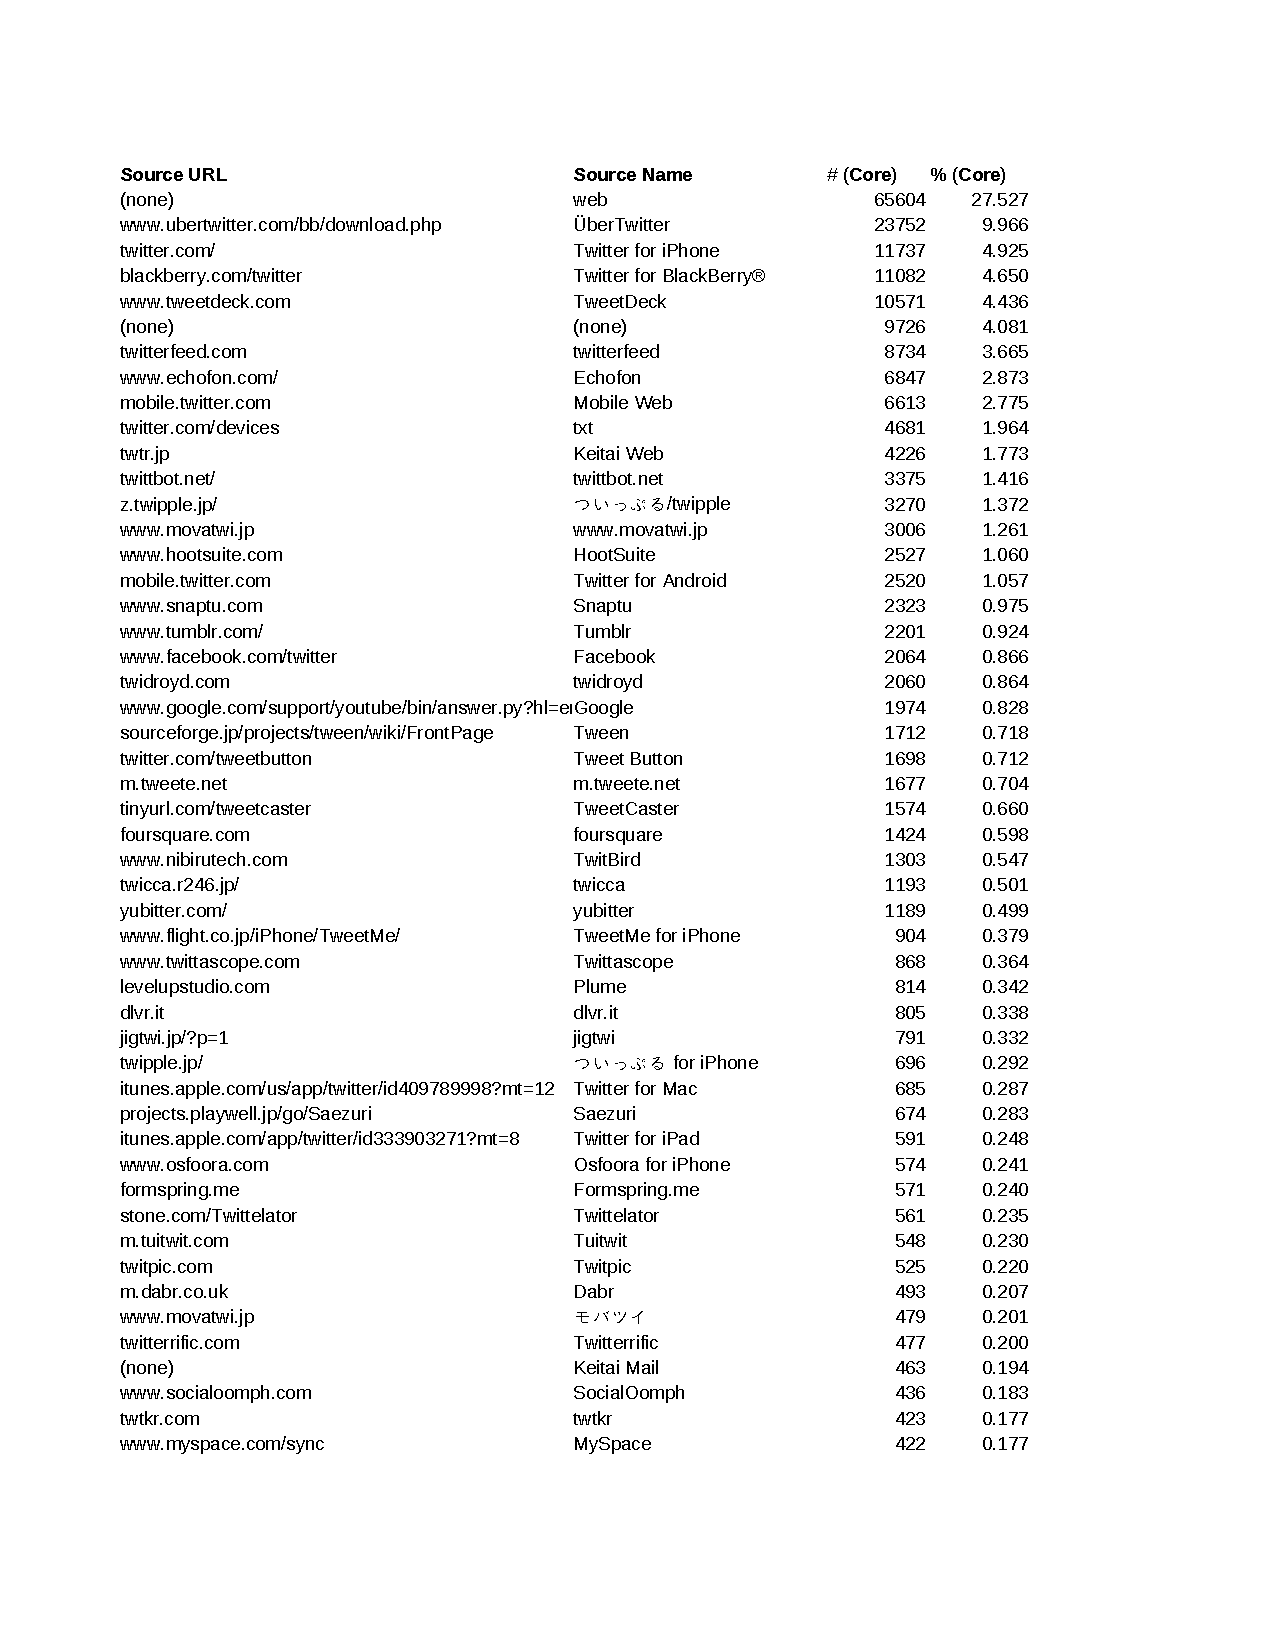
\includegraphics[width=6in,bb=0 0 612 792,keepaspectratio=true]{./sources.pdf}
% sources.pdf: 612x792 pixel, 72dpi, 21.59x27.94 cm, bb=0 0 612 792

\twocolumn
\subsection{Location}
\noindent Location data is entered free-form.  That is, a user can set their location field to anything they want.  In order to use the location data, we need to figure out which locations are not valid, and we need to transform valid locations into a format that can be processed.  For example, we want all users from San Francisco to have a location attribute of \textit{San Francisco, CA, USA}, so that we can easily determine which users share a location.  We are using the Google Maps Geocoding API to make this conversion.  When the API returns more than one result, we can either remove those location from our analysis, try a different method of processing, or try to determine the commonality between multiple results (if, for example, all results are in France, we can use France in our analysis).  When the API returns zero results, we cannot use the location data.\\\\
The Geocoding API has some amount of error.  The returned results are not always a correct transformation of the original location.  We cannot manually examine each result for error, but we do plan to look at a subset of the results and derive a general error rate from that sample.\\\\
The Geocoding API is rate-limited to 2,500 queries per day per IP address.  Google Maps API Premier members can query up to 100,000 per day, but that service starts at \$10,000, so is probably beyond the budget of this project. Yahoo also has a Geocoding API, to which we can make 5,000 calls per day.  However, we would prefer not to complicate the data collection by using both Google and Yahoo services.\\\\
Rate-limiting of Geocoding queries is an issue we need to address urgently.  We either need to find a way to make more requests to the API without breaking the terms of service, or we need to get the information from the Google or Yahoo front-end.  Alternatively, we could design our own location-conversion script, but we see this as non-ideal.



\twocolumn
\bibliography{citations}
\end{document}
